\chapter{مفاهیم پایه‌ای}
\label{chap:concepts}
در این بخش به مرور مفاهیم بنیادی پرداخته می‌شود که در ادامه و در بررسی پژوهش‌های گذشته در بخش 
\autoref{chap:related}
به فهم عمیق‌ و درک اساس آن‌ها کمک می‌کند. این مفاهیم عبارتند از مبانی یادگیری ژرف، روش گسترش ژرف، دانش‌دامنه و یادگیری ژرف در شبکه‌های بی‌سیم.
\section{مبانی یادگیری ژرف}
هوش مصنوعی با آزمون معروف تورینگ در دهه‌ی ۱۹۵۰ آغاز شد که نقطه‌ی عطفی در توانایی تفکر ماشینی محسوب می‌شود. در طول دهه‌ها، و به‌ویژه در دهه‌ی ۱۹۹۰، یادگیری ماشین به‌عنوان زیرشاخه‌ای از هوش مصنوعی شکل گرفت. یادگیری ماشین نیازمند استخراج دستی ویژگی‌ها از داده‌های ساخت‌یافته است. بیشتر الگوریتم‌های یادگیری ماشین را می‌توان در سه دسته‌ی یادگیری نظارت‌شده، یادگیری بدون نظارت، و یادگیری تقویتی تقسیم‌بندی کرد.
\begin{figure}
	\centering
	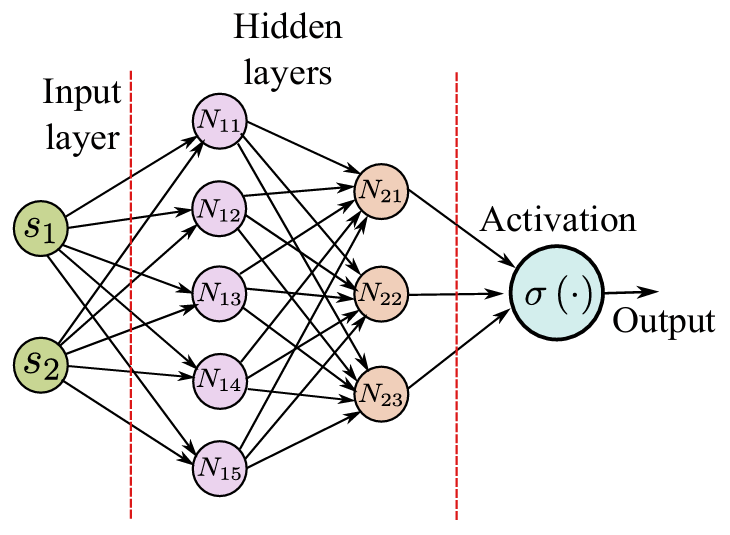
\includegraphics[width=0.5\linewidth]{./Pic/ComprehensiveReview_concepts_fig1}
	\caption[\lofimage{./Pic/ComprehensiveReview_concepts_fig1} ساختار شبکه‌ عصبی پیش‌خور]{ساختار شبکه‌ی عصبی پیش‌خور \cite{ComprehensiveReview}}
	\label{concepts:fig1}
\end{figure}
در یادگیری نظارت‌شده، هدف این است که مدل بیاموزد چگونه ورودی‌ها را به خروجی‌ها نگاشت کند تا بتواند برچسب داده‌های جدید را پیش‌بینی کند. در یادگیری بدون نظارت، مجموعه‌داده شامل ویژگی‌های بسیاری است که دارای برچسب نیستند. الگوریتم تلاش می‌کند تا الگوهای پنهان در داده را بدون راهنمایی نمونه‌های برچسب‌دار شناسایی کند. دسته‌ی سوم، یادگیری تقویتی است که شامل عاملی می‌شود که بر اساس تعامل با محیط می‌آموزد تصمیم‌گیری کند. از آن‌جا که مجموعه‌داده‌ی از پیش تعیین‌شده‌ای وجود ندارد، عامل با محیط تعامل کرده و از بازخوردهایی که در نتیجه‌ی هر عمل دریافت می‌کند، یاد می‌گیرد.
خروجی یک الگوریتم یادگیری ماشین می‌تواند دو نوع باشد: 
\gls{Regression}
 و 
\gls{Classification}.

در دهه‌ی اول ۲۰۰۰، یادگیری ژرف به‌عنوان فناوری‌ای کلیدی در طراحی شبکه‌های هوشمند با داده‌های غیرساخت‌یافته ظهور کرد. پژوهشگران از روش‌های یادگیری ژرف برای حل مسائل پیچیده استفاده کرده‌اند. این روش به‌طور گسترده در بینایی ماشین، پردازش زبان طبیعی و پردازش تصویر به‌کار رفته است. موفقیت آن الهام‌بخش پژوهشگران شد تا از یادگیری ژرف در لایه‌ی فیزیکی شبکه‌های ارتباط بی‌سیم نیز استفاده کنند، به‌ویژه در زمینه‌ی وظایف مختلف پردازش سیگنال.

یک شبکه‌ی عصبی مصنوعی از لایه‌های به‌هم‌پیوسته‌ای از نورون‌ها تشکیل شده است که با همکاری یکدیگر می‌آموزند تا الگوهایی را از داده‌های ورودی استخراج کنند. انواع گوناگونی از معماری‌های شبکه‌های عصبی برای وظایف مختلف یادگیری توسعه یافته‌اند، از جمله: 
\glspl{Feedforward Neural Network}،
\glspl{Convolutional Neural Network}،
\glspl{Recurrent Neural Network}
 و 
\gls{Graph Neural Network}.
\autoref{concepts:fig1}
 معماری یک شبکه‌ی عصبی پیش‌خور با 
$K$
(در این‌جا 
$K=2$)
لایه‌ی پنهان و
$N_{k}$
نورون در هر لایه‌ی 
$k$
(برای همه‌ی
$k = 0,...,K$) 
     را نشان می‌دهد. این معماری شامل سه بخش اصلی است: لایه‌ی ورودی، لایه‌های پنهان و لایه‌ی خروجی.
اکنون مراحل عملکرد یک شبکه‌ی عصبی پیش‌خور را بررسی می‌کنیم:
\begin{enumerate}
\item 
شبکه با یک بردار ورودی
$\bold{s} = [s_{1}, s_{2}, ..., s_{n}]$،
در لایه ورودی آغاز می‌شود، که در آن 
$n$
تعداد ویژگی‌های ورودی است.
\item
برای هر نورون در یک لایه، جمع وزن‌دار ورودی‌ها محاسبه می‌شود:
\begin{equation}
	z_{j}^{(k)} = \sum_{i=1}^{n} \omega_{ji}^{(k)} s_j + b_{j}^{(k)} ,
\end{equation}
که در آن 
$\omega_{ji}^{(k)}$
وزن اتصال نورون
$i$
به نورون
$j$
در لایه
$k$
است و
$b_{j}^{(k)}$
سوگیری نورون
$j$
در همان لایه است.
\item 
یک تابع فعال‌سازی غیرخطی
$\sigma(0)$
بر روی خروجی اعمال می‌شود:
\begin{equation}
a_{j}^{(k)} = \sigma(z_{j}^{(k)}) ,
\end{equation}
که در آن
$a_{j}^{(k)}$
خروجی فعال‌شده‌ی نورون
$j$
در لایه 
$k$
است. تابع‌های فعال‌سازی رایج شامل
\lr{ReLU}،
\lr{sigmoid}،
\lr{tanh}
 و
\lr{softmax}
هستند.
\item 
در لایه‌ی خروجی، پس از انجام جمع وزن‌دار و تابع فعال‌سازی، خروجی نهایی به‌صورت زیر به‌دست می‌آید:
\begin{equation}
	\hat{y} = \sigma(\bold{W}^{K}\bold{s}^{K} + \bold{b}^{K})
\end{equation}
که در آن
$\bold{K}$
ماتریس وزن‌ها و
$\bold{b}$
بردار سوگیری در لایه خروجی است. تابع فعال‌سازی در این مرحله بسته به نوع مسئله (طبقه‌بندی یا رگرسیون) انتخاب می‌شود.
\item
سپس 
\gls{Loss Function}
برای اندازه‌گیری عملکرد شبکه محاسبه می‌شود:
\begin{equation}
	\mathcal{L}(\hat{\bold{y}},\bold{y})
\end{equation}
که در آن
$\bold{\hat{y}}$
خروجی پیش‌بینی‌شده و
$\bold{y}$
خروجی واقعی است.
تابع‌های زیان رایج شامل میانگین مربعات خطا 
(\gls{MSE})،
\gls{Binary Cross-Entropy}
و 
\gls{Categorical Cross-Entropy}
هستند.
برای آموزش شبکه‌ی عصبی، از روش 
\gls{Backpropagation}
استفاده می‌شود. در این فرآیند، پارامترهای شبکه (وزن‌ها و سوگیری‌ها) به‌گونه‌ای تنظیم می‌شوند که مقدار خطا به حداقل برسد. پارامترها معمولاً با الگوریتم‌های بهینه‌سازی مانند گرادیان کاهشی تصادفی 
(\gls{SGD})
به‌روزرسانی می‌شوند.
\end{enumerate}

در مقابل، شبکه‌های عصبی پیچشی برای پردازش 
\glspl{Grid-like Data}
مانند تصویر طراحی شده‌اند و از ساختار فضایی داده‌ها بهره می‌برند. این شبکه‌ها از لایه‌های پیچشی برای استخراج ویژگی‌هایی مانند لبه‌ها استفاده می‌کنند و سپس با 
\glspl{Pooling Layer}
ابعاد فضایی را کاهش داده و اطلاعات کلیدی را حفظ می‌کنند. ویژگی‌های استخراج‌شده سپس به 
\glspl{Fully Connected Layer}
منتقل می‌شوند.
یکی از نخستین کاربردهای، طبقه‌بندی مدولاسیون بر اساس 
\gls{Signal Constellation Diagram}
بود، که در آن پژوهشگران از روش یادگیری ژرف مبتنی بر شبکه‌های عصبی پیچشی استفاده کردند. آن‌ها روش‌هایی برای نمایش سیگنال‌های مدوله‌شده در قالب داده‌های شبکه‌ای متناسب با معماری 
\gls{CNN}
توسعه دادند.

\gls{Recurrent Neural Network}
نوع دیگری از شبکه‌های عصبی هستند که به‌طور خاص برای پردازش داده‌های توالی‌دار طراحی شده‌اند. در 
\gls{RNN}،
خروجی هر مرحله به‌عنوان ورودی مرحله‌ی بعد استفاده می‌شود و به این ترتیب وابستگی‌های زمانی و ترتیبی میان گره‌ها حفظ می‌گردد. این کار توسط نورون بازگشتی که یک حالت پنهان را نگه می‌دارد انجام می‌شود.
یکی از نسخه‌های مشهور 
\gls{RNN}،
\gls{LSTM}
است. شبکه‌ی 
\gls{LSTM}
در چارچوب 
\gls{NOMA}
برای یادگیری ویژگی‌های کانال سامانه 
\gls{NOMA}
مورد استفاده قرار گرفته است.
\gls{Deep Reinforcement Learning}
ترکیبی از 
\gls{Reinforcement Learning}
و 
\gls{Deep Learning}
است که با هدف توسعه‌ی 
\gls{Agent}های
هوشمندی طراحی شده که قادرند در محیط‌های پیچیده تصمیم‌های متوالی اتخاذ کنند. در 
\gls{Deep Reinforcement Learning}،
عامل با محیط تعامل می‌کند تا 
\gls{Cumulative Reward}
را بیشینه کند و از طریق اکتشاف و بهره‌برداری سیاست‌های بهینه را بیاموزد.
در این میان، 
\glspl{Deep Neural Network}
برای تقریب 
\glspl{Value Function}
یا 
\glspl{Policy}
به‌کار می‌روند تا 
\gls{Deep Reinforcement Learning}
بتواند با فضاهای حالت و عمل با ابعاد بالا کار کند.

روش‌های کلیدی مانند 
\gls{DQN}،
\glspl{Policy Gradient Method}
و چارچوب‌های Actor-Critic به عامل‌ها اجازه می‌دهند عملکرد خود را از طریق آزمون و خطا و براساس سیگنال‌های پاداش به‌تدریج بهبود دهند.
در حوزه‌ی ارتباطات و شبکه‌ها، 
\gls{Deep Reinforcement Learning}
 به‌عنوان ابزاری قدرتمند برای حل چالش‌هایی مانند تخصیص منابع، مدیریت طیف و بهینه‌سازی شبکه مطرح شده است.
معماری‌های مدرن شبکه مانند اینترنت اشیا، شبکه‌های ناهمگن 
(\gls{HetNet})
 و شبکه‌های پهپادی 
(\gls{UAV})
  دارای ویژگی‌هایی غیرمتمرکز، پویا و خودکار هستند، که آن‌ها را برای راهکارهای مبتنی بر یادگیری تقویتی بسیار مناسب می‌سازد.

مفهوم استفاده از 
\glspl{Autoencoder}
 برای طراحی 
\gls{End-to-End Communication System}
به‌طور گسترده مورد مطالعه قرار گرفته است. در این نوع یادگیری، یک مدل واحد آموزش داده می‌شود تا ورودی خام را مستقیماً به خروجی مطلوب نگاشت کند، بدون نیاز به مراحل میانی یا استخراج ویژگی دستی.
در این چارچوب، 
\gls{Autoencoder}
 هر دو بخش فرستنده و گیرنده را به‌صورت هم‌زمان بهینه‌سازی می‌کنند. هدف در سامانه‌های ارتباطی، طراحی مشترک فرستنده و گیرنده برای یک مدل کانال مشخص است، که این کار منجر به بهبود عملکرد، همگرایی سریع‌تر و نرخ خطای بیت کمتر می‌شود.

شبکه‌های عصبی گرافی برای داده‌های ساختار یافته به‌صورت گراف طراحی شده‌اند، جایی که گره‌ها توسط یال‌ها به هم متصل‌اند. برخلاف شبکه‌های عصبی مرسوم، 
\lr{GNN}ها
روی داده‌های 
\gls{Non-Euclidean}
عمل می‌کنند و روابط بین گره‌ها را در گراف مدل می‌کنند.
آن‌ها با تجمیع و تبدیل ویژگی‌ها از گره‌های همسایه، نمایش‌های غنی از گره‌ها، یال‌ها یا کل گراف را می‌آموزند. این قابلیت، 
\lr{GNN}ها
را در انجام وظایفی که به داده‌های رابطه‌ای وابسته‌اند، بسیار کارآمد می‌کند.

در سال ۲۰۲۰، گودفلو و همکارانش الگوریتم جدیدی برای
\gls{Generative Modeling}
معرفی کردند. این الگوریتم، معروف به 
\gls{Generative Adversarial Network}،
از دو شبکه‌ی عصبی تشکیل شده است:
یک 
\gls{Generator}
که خروجی‌های واقع‌گرایانه تولید می‌کند، و یک 
\gls{Discriminator}
که تشخیص می‌دهد داده‌ها واقعی هستند یا ساختگی.
با رقابت و یادگیری هم‌زمان میان این دو شبکه، 
\lr{GNN}ها
قادر به تولید داده‌هایی با کیفیت بالا هستند که اغلب از داده‌های واقعی قابل‌تمایز نیستند.

\section{سازوکار گسترش ژرف}
روش 
\gls{Deep Unfolding}
یک روش معمول در حوزه‌ی 
\gls{Model-Driven Deep Learning}
است. این روش به‌طور گسترده برای وظایفی مانند 
\gls{Signal Detection}،
 طراحی ماتریس‌های 
\gls{Beamforming}
 و بسیاری از مسائل بهینه‌سازی در ارتباطات بی‌سیم مورد استفاده قرار گرفته است.

به دلیل کاهش زمان آموزش و نیاز کمتر به داده‌های آموزشی، 
\gls{Deep Unfolding}
به‌عنوان یک رویکرد جایگزین امیدوارکننده نسبت به روش‌های صرفاً مبتنی بر مدل یا صرفاً مبتنی بر داده مطرح شده است. در واقع، 
\gls{Deep Unfolding}
تلفیقی از رویکردهای مبتنی بر مدل و 
\gls{Domain Knowledge}
را در طراحی معماری 
\gls{Deep Neural Network}
به‌کار می‌گیرد.

فرآیند آموزش در این روش به‌صورت انتها به انتها انجام می‌شود. در 
\gls{Deep Unfolding}،
یک 
\gls{Iterative Algorithm}
به لایه‌های 
\gls{Deep Neural Network}
نگاشت می‌شود. سپس از روش‌های 
\gls{Deep Learning}
 مانند 
\gls{SGD}
 برای یادگیری پارامترها استفاده می‌شود.
\begin{figure}
	\centering
	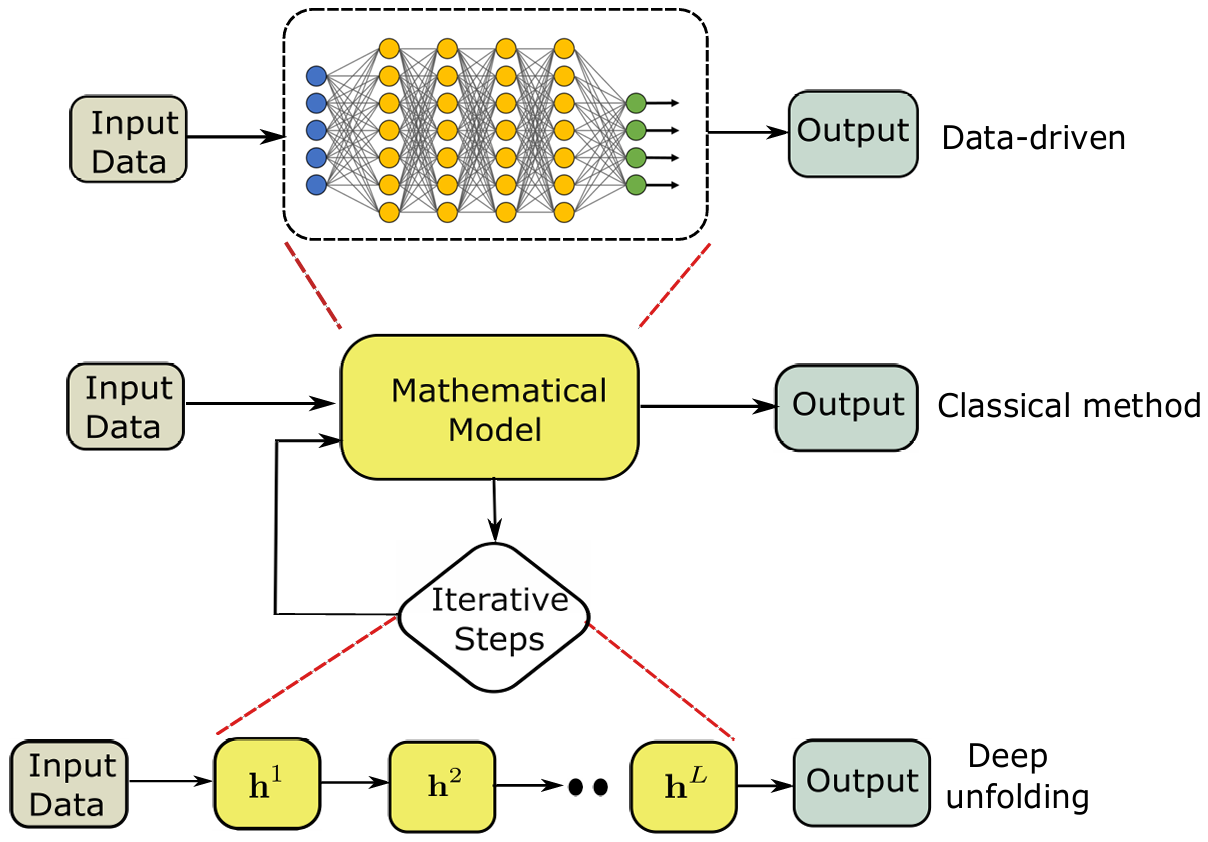
\includegraphics[width=0.5\linewidth]{./Pic/ComprehensiveReview_concepts_fig2}
	\caption[\lofimage{./Pic/ComprehensiveReview_concepts_fig2} طرح‌واره‌ای از رویکردهای داده-محور، مرسوم و گسترش ژرف]{طرح‌واره‌ای از رویکردهای داده-محور، مرسوم و گسترش ژرف \cite{ComprehensiveReview}}
	\label{concepts:fig2}
\end{figure}

\autoref{concepts:fig2}
 نموداری طرح‌واره‌ای از مقایسه‌ی سه رویکرد مرسوم، داده-محور و گسترش ژرف را نشان می‌دهد. همچنین  
\autoref{concepts:fig3}
  نمایی دقیق‌تر از نحوه‌ی عملکرد رویکرد
\gls{Deep Unfolding}
   را ارائه می‌دهد.
برای هر الگوریتم تکرارشونده، معادله‌ی به‌روزرسانی در هر تکرار به‌صورت زیر بیان می‌شود:
\begin{equation}
	\bold{s}^{(t+1)} = h(\bold{s}^{t};\bold{\Psi}^{t})
	\label{concepts:eq1}
\end{equation}
در 
\autoref{concepts:eq1}،
$\bold{s}^{t}\in\mathbb{R}^{n}$
بردار متغیری است که در هر تکرار باید به‌روزرسانی شود و
$t = 1,...,T$
نشان‌دهنده‌ی شماره‌ی تکرار است. تابع تکرارشونده‌ی الگوریتم با
$h(\cdot; \cdot): \mathbb{R}^n \rightarrow \mathbb{R}^n$
پارامترهای قابل یادگیری
$\bold{\Psi}_t \in \mathbb{R}^n$
شامل پارامترهای مدل و گام‌های تنظیم ضرایب منظم‌سازی در الگوریتم هستند. هر تابع تکرارشونده‌ی
$h(\cdot;\cdot)$
به یک لایه‌ی شبکه‌ی عصبی نگاشت می‌شود، و چندین لایه از این نوع به‌صورت پشته‌ای در کنار هم قرار می‌گیرند (مطابق 
\autoref{concepts:fig2}).
برای یادگیری پارامترهای قابل آموزش
$\bold{\Psi}^t$
در یک رویکرد انتها به انتها، بهینه‌سازی زیر انجام می‌شود:
\begin{equation}
	minimize_{\bold{\Psi}_T} \; \mathcal{L}\big(\bold{s}^T(\bold{\Psi}_T)\big)
\end{equation}
که در آن 
$\mathcal{L}(\cdot)$
تابع زیان برای آموزش است و
$\bold{\Psi}_T = \{ \Psi^t \}_{t=0}^{T}$
مجموعه‌ی همه‌ی پارامترهای قابل یادگیری در شبکه‌ی دارای
$T$
لایه است، در حالی که 
$\bold{s}^{T}(\cdot)$
خروجی شبکه‌ی گسترش‌یافته است.
\begin{figure}
	\centering
	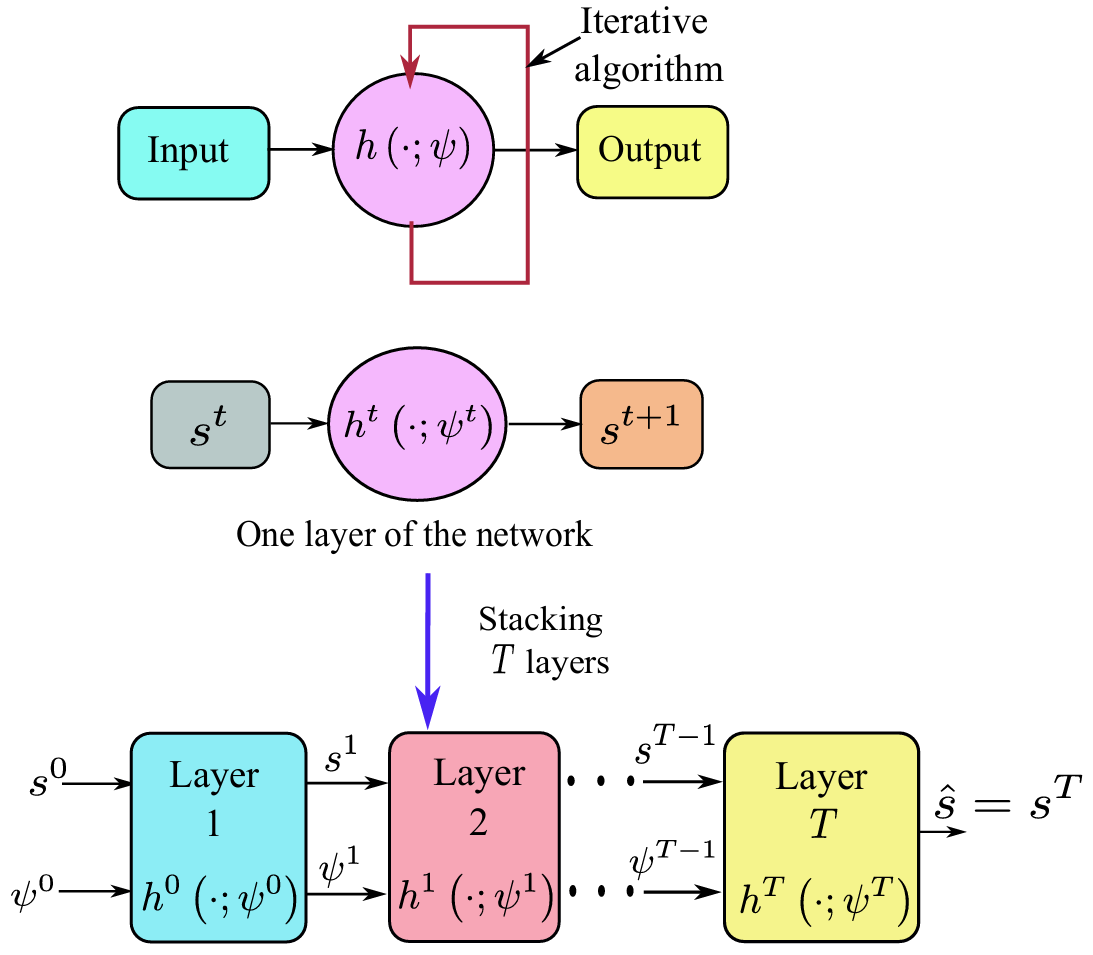
\includegraphics[width=0.5\linewidth]{./Pic/ComprehensiveReview_concepts_fig3}
	\caption[\lofimage{./Pic/ComprehensiveReview_concepts_fig3} چارچوب کلی گسترش ژرف]{چارچوب کلی گسترش ژرف \cite{ComprehensiveReview}}
	\label{concepts:fig3}
\end{figure}
عبور داده از شبکه‌ گسترش‌یافته با پارامترهای آموزش‌دیده در مرحله‌ی آزمایش مشابه اجرای همان الگوریتم تکرارشونده بهینه‌شده از نظر پارامترها برای تعداد محدودی از تکرارها است. بنابراین، تعداد لایه‌ها در مدل‌های 
\gls{Deep Unfolding}
 ثابت بوده و در نتیجه پیچیدگی محاسباتی از پیش تعیین‌شده‌ای دارد. در درون این لایه‌های ثابت، مدل آموزش می‌بیند تا پارامترهای قابل یادگیری را بهینه کند و مسئله را از طریق یک الگوریتم ساخت‌یافته با پارامترهای تنظیم‌شده برای دستیابی به عملکرد بهینه حل نماید.

مراحل حل یک مسئله‌ی بهینه‌سازی با استفاده از رویکرد
\gls{Deep Unfolding}
در ادامه آمده است.
\begin{enumerate}
	\item 
انتخاب الگوریتم اصلی: ابتدا الگوریتم پایه‌ای شناسایی شده که اساس طراحی 
\gls{Deep Unfolding}
 خواهد بود.
\item
انتخاب پارامترهای قابل یادگیری:
برخی از پارامترها یا بلوک‌های خاص در الگوریتم اصلی را انتخاب کرده و آن‌ها را با عملیات داده‌محور آموزش‌پذیر جایگزین می‌شود.
\item
تعریف تابع خطا و نمایش الگوریتم به‌صورت شبکه‌ی عصبی:
هر لایه در شبکه متناظر با یک تکرار از الگوریتم اصلی است. شبکه سپس با استفاده از روش‌های نظارتی یا بدون نظارت آموزش داده می‌شود. از آن‌جا که تعداد تکرارها از پیش تعیین شده است، تعداد لایه‌های شبکه نیز با آن برابر است. در صورت نیاز، تعداد لایه‌ها می‌تواند تنظیم شود تا میان عملکرد و پیچیدگی محاسباتی تعادل برقرار گردد.
\end{enumerate}
الگوریتم‌های اصلی معمولاً تکرارشونده و مبتنی بر روش‌های بهینه‌سازی هستند، اما غالباً پیچیده، محاسباتی سنگین و کند در همگرایی هستند. 
\gls{Deep Unfolding}
 این الگوریتم‌ها را از طریق آموزش داده‌محور بهبود می‌دهد. مزایا و دستاوردهای کلیدی 
\gls{Deep Unfolding}،
بهینه‌سازی
\glspl{Hyperparameter}
 برای افزایش سرعت همگرایی و ساده‌سازی وظایف پیچیده مانند وارون‌سازی یا تجزیه‌ی ماتریسی، با پیچیدگی محاسباتی کمتر هستند.
کاربرد نخست به‌ویژه در روش‌های
\gls{Unfolded Projected Gradient Ascent/Descent}
(\gls{PGA}/\gls{PGD})
 رایج است، در حالی‌که کاربرد دوم به‌طور گسترده در 
\gls{Unfolded Weighted Minimum Mean Square Error}
  مورد استفاده قرار می‌گیرد. رویکرد دیگری نیز وجود دارد که شامل یادگیری خروجی در هر لایه است، که متناظر با حل هر تکرار الگوریتم اصلی است. این روش در 
\glspl{Detection Network}،
 به‌ویژه بر پایه‌ی چارچوب PGA/PGD، به‌طور گسترده به‌کار گرفته شده است.

برتری اساسی 
\gls{Deep Unfolding}
 در این است که می‌تواند
\gls{Domain Knowledge}
  را مستقیماً در ساختار شبکه‌ی عصبی ادغام کند. این ویژگی باعث می‌شود شبکه با تعداد پارامتر کمتر و لایه‌های ثابت عملکرد بهتری ارائه دهد و در عین حال پیچیدگی را کاهش دهد.
در نتیجه، 
\gls{Deep Unfolding}
نسبت به 
\gls{Generic Deep Neural Network}
به مجموعه‌داده‌ی آموزشی کوچکتری نیاز دارد.

\section{دانش دامنه و یادگیری ژرف در شبکه‌های بی‌سیم}
در این بخش با ارائه تعریفی روشن از دانش در حوزه شبکه‌های بی‌سیم شروع می‌کنیم. متعاقباً، این دانش حوزه خاص ارتباطات را به دو دسته کلی، یعنی دانش علمی و دانش تخصصی، طبقه‌بندی می‌کنیم. در هر دسته، انواع دانش خاص‌تر و همچنین بازنمایی‌ها و نمونه‌های معمول مربوط به آنها، به تفصیل ارائه شده است.

‫درک مفاهیم پایه در حوزه شبکه‌های بی‌سیم هوشمند، به‌ویژه در نسل‌های آتی مانند نسل ششم، نیازمند فهم عمیق در خصوص چیستی 
\gls{Domain Knowledge}
، ساختارهای نوین 
\gls{Deep Learning}
و چگونگی ادغام این دو نظام فکری از طریق روش‌های مدل‌محور مانند 
\gls{Deep Unfolding}
 است. این بخش به تشریح این اصول می‌پردازد.‬
نخست، مفهوم و طبقه‌بندی دانش در شبکه‌های بی‌سیم‬ است.
‫دانش به معنای شناخت و خلاصه‌ای از نتایج اکتشافات بشری درباره جهان فیزیکی و ذهنی است که از دنیای واقعی کشف شده و سپس به عنوان اصول راهنما برای بهبود جهان به کار می‌رود. تعریف دقیق و یکنواخت دانش آسان نیست، زیرا دارای ماهیت انتزاعی و تعمیم‌یافته است و حتی در حوزه معرفت‌شناسی فلسفی همچنان موضوعی بحث‌برانگیز است. تعریف مرسوم ارائه شده توسط افلاطون بیان می‌کند که برای واجد شرایط بودن به عنوان دانش، یک گزاره باید سه معیار توجیه‌پذیری، حقیقی بودن و باورپذیری را برآورده کند. یک مفهوم جهانی‌تر از دانش، انباشت شناخت و تجربیات فردی است که از طریق فعالیت‌های عملی با هدف تغییر جهان عینی جمع‌آوری می‌شود و شامل درک ماهیت، ویژگی‌ها و حالات اشیا و همچنین روش‌های حل مسئله است. در هوش مصنوعی، دانش اغلب به توصیف روابط بین موجودیت‌ها در زمینه‌های خاص می‌پردازد و از طریق تجزیه و تحلیل مجموعه‌ای از اطلاعات به دست می‌آید.‬

‫برای شبکه‌های بی‌سیم، 
\gls{Communication-specific domain knowledge}
به عنوان نظریه‌های فنی و شناخت تجربی تعریف می‌شود که توسط دانشمندان و متخصصان در فرآیند طراحی، ساخت و بهینه‌سازی شبکه‌های ارتباطی بی‌سیم انباشته شده است. این دانش دو جنبه محوری دارد. اوّل، در طول فرآیند مدل‌سازی، شامل توصیف شناختی ویژگی‌ها و قوانین تکاملی محیط شبکه و الزامات خدمت است همچون مدل‌سازی وظایف بی‌سیم مانند 
\gls{Markov Decision Process}.
 دوم، در طول فرآیند تصمیم‌گیری، خلاصه‌ای شناختی از اصول، الگوریتم‌ها و نظریه‌های مدل‌محور است که در حل مسئله به کار می‌روند مانند الگوریتم‌های نظری برای تخصیص توان.‬

\begin{figure}
	\centering
	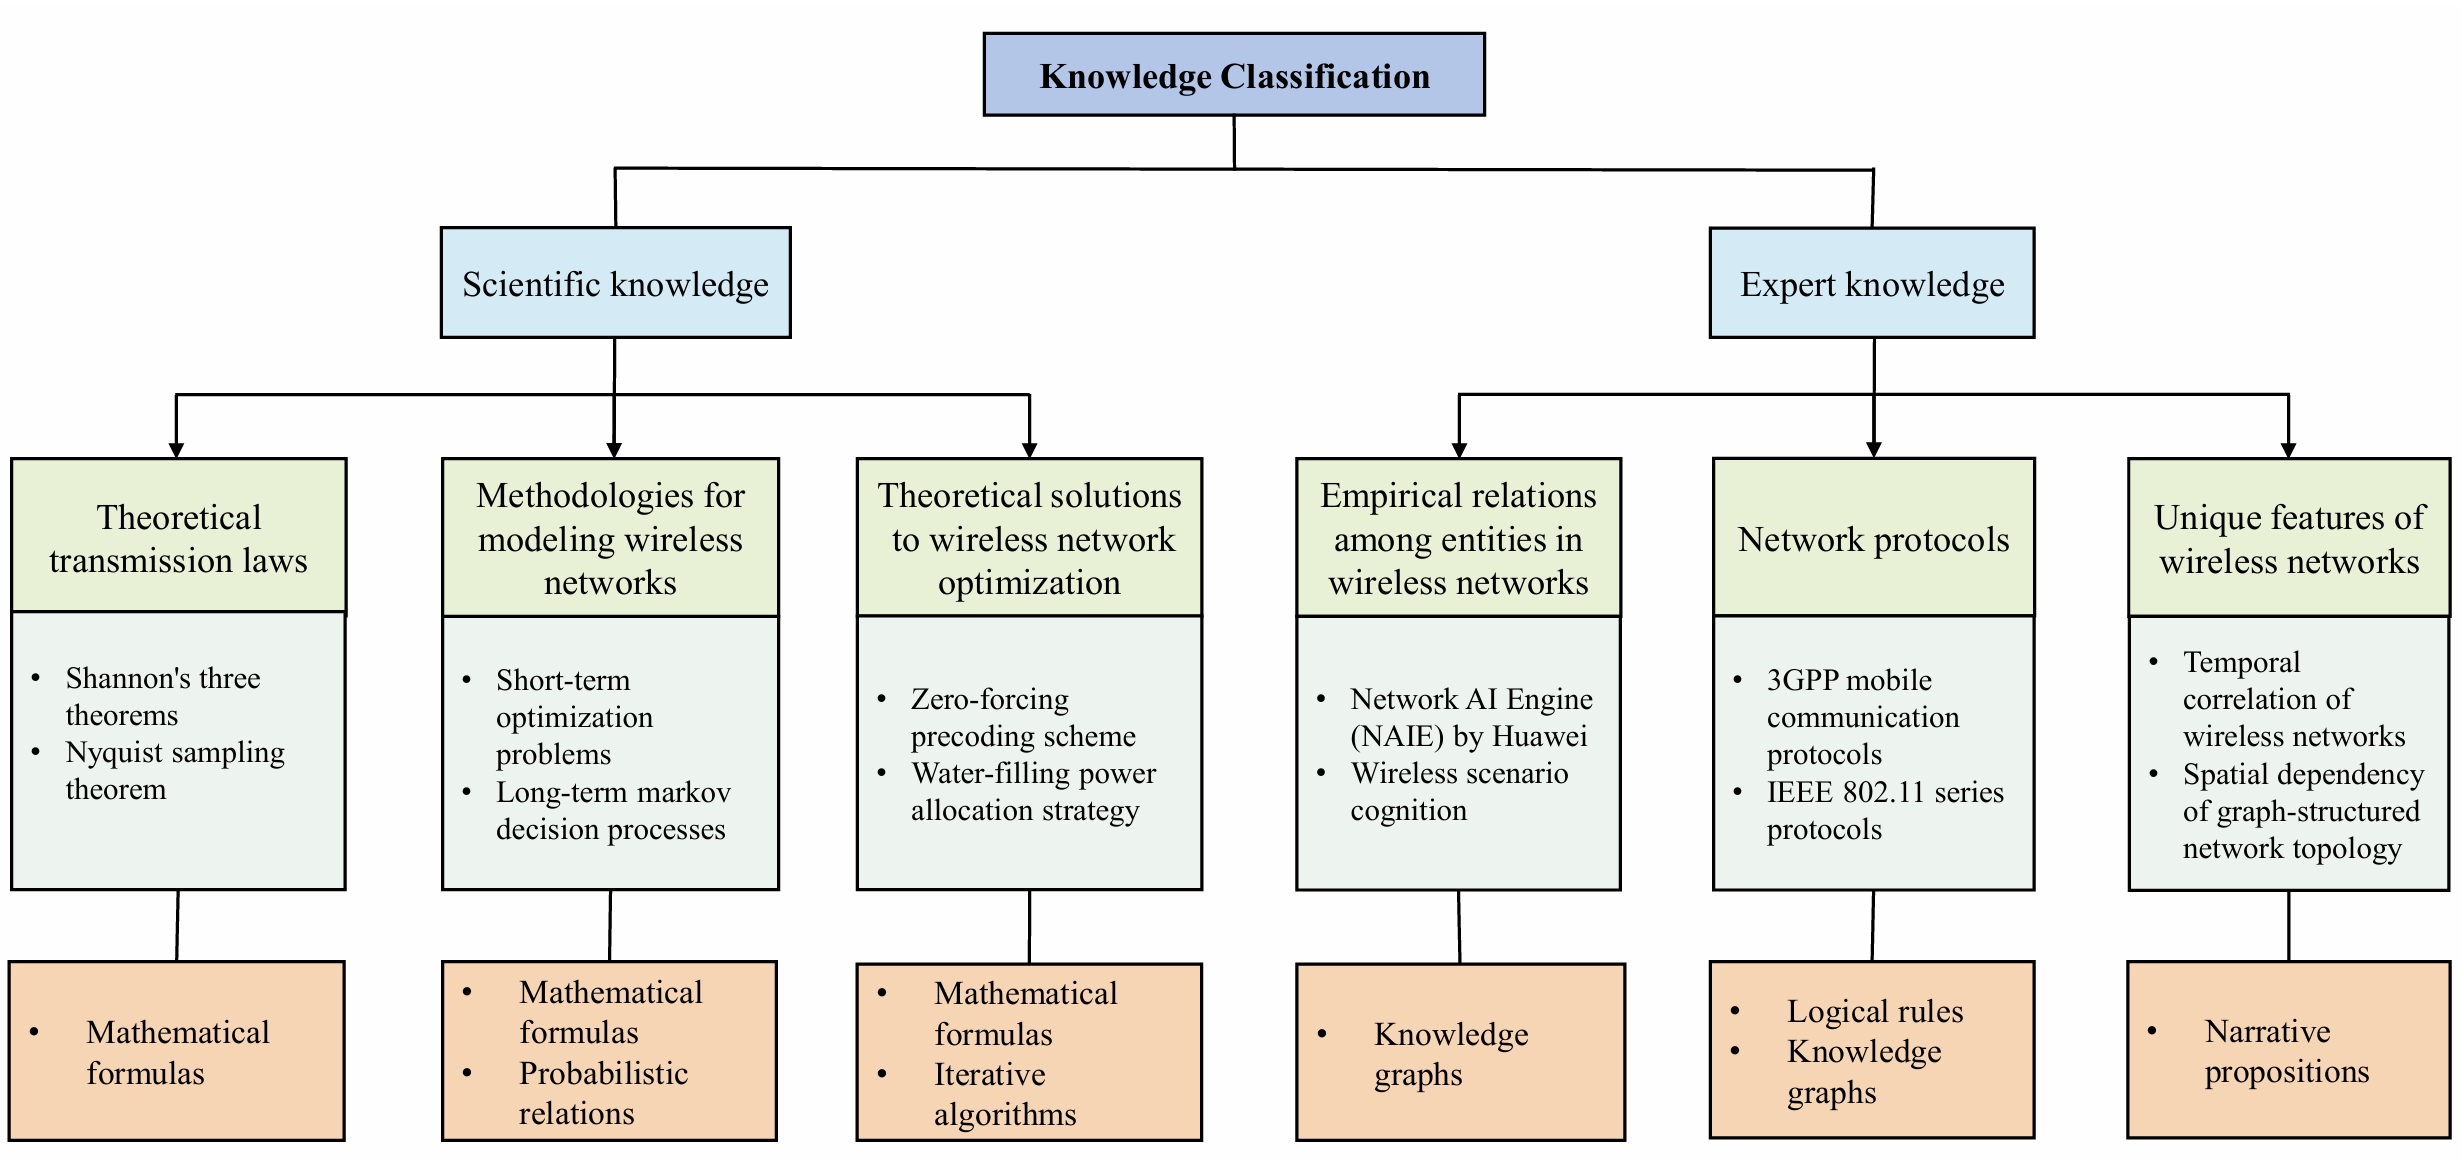
\includegraphics[width=0.9\linewidth]{./Pic/ComprehensiveSurvey_concepts_fig4}
	\caption[\lofimage{./Pic/ComprehensiveSurvey_concepts_fig4} طبقه‌بندی دانش در شبکه‌های بی‌سیم شامل، دسته‌بندی دانش، نمایش‌دانش و مثال‌های رایج]{طبقه‌بندی دانش در شبکه‌های بی‌سیم شامل، دسته‌بندی دانش، نمایش‌دانش و مثال‌های رایج\cite{ComprehensiveSurvey}}
	\label{concepts:fig4}
\end{figure}
‫دانش دامنه مطابق
\autoref{concepts:fig4}
 به دو دسته کلی دانش علمی و دانش تخصصی طبقه‌بندی می‌شود. این تمایز برای تفکیک پایه‌های بنیادی، اشکال نمایش و نقش‌های عملکردی آن‌ها در 
\gls{Knowledge-Driven Deep Learning}
حیاتی است. دانش علمی با هدف ایجاد قوانینی جهانی است که سازوکار عملکرد شبکه‌های بی‌سیم را به صورت نظری توضیح می‌دهد. این دانش، نظام‌مند و عینی است و معمولاً به صورت صریح در قالب فرمول‌های ریاضی رسمی، الگوریتم‌ها و روابط احتمالی بیان می‌شود. در مقابل، دانش تخصصی به تجربیات عملی یا شهود اشاره دارد که توسط متخصصان و مهندسان در طول زمان خلاصه و اعتبارسنجی شده است. این دانش متنی، ذهنی و اغلب در عبارات نسبتاً غیررسمی مانند نمودارهای دانش یا گزاره‌های روایی ارائه می‌شود.‬

دسته‌بندی دیگر 
\gls{Deep Neural Network}
 و نظام فکری 
\gls{Knowledge-Driven Deep Learning}‬
است. 
\gls{Deep Learning}
که یک فناوری حیاتی در دهه اخیر است، بر پایه 
\gls{Deep Neural Network}
 بنا شده است. مدل‌های 
\gls{Deep Learning}
  شامل معماری‌های مختلفی هستند که باید بر اساس ویژگی‌های مسئله مورد نظر انتخاب شوند. برای مثال، دانش مربوط به همبستگی‌های زمانی ترافیک بی‌سیم یا وابستگی زمانی ناشی از 
\gls{Inter Symbol Interference}
   در آشکارسازی سیگنال، استفاده از 
\gls{Recurrent Neural Network}
    یا 
\gls{Long Short-Term Memory}
    را هدایت می‌کند. همچنین، دانش درباره وابستگی فضایی و ساختار گرافی توپولوژی شبکه بی‌سیم، انتخاب 
\gls{Graph Neural Network}
     را برای مسائلی مانند تخصیص توان توجیه می‌کند.‬
 \begin{figure}
   	\centering
   	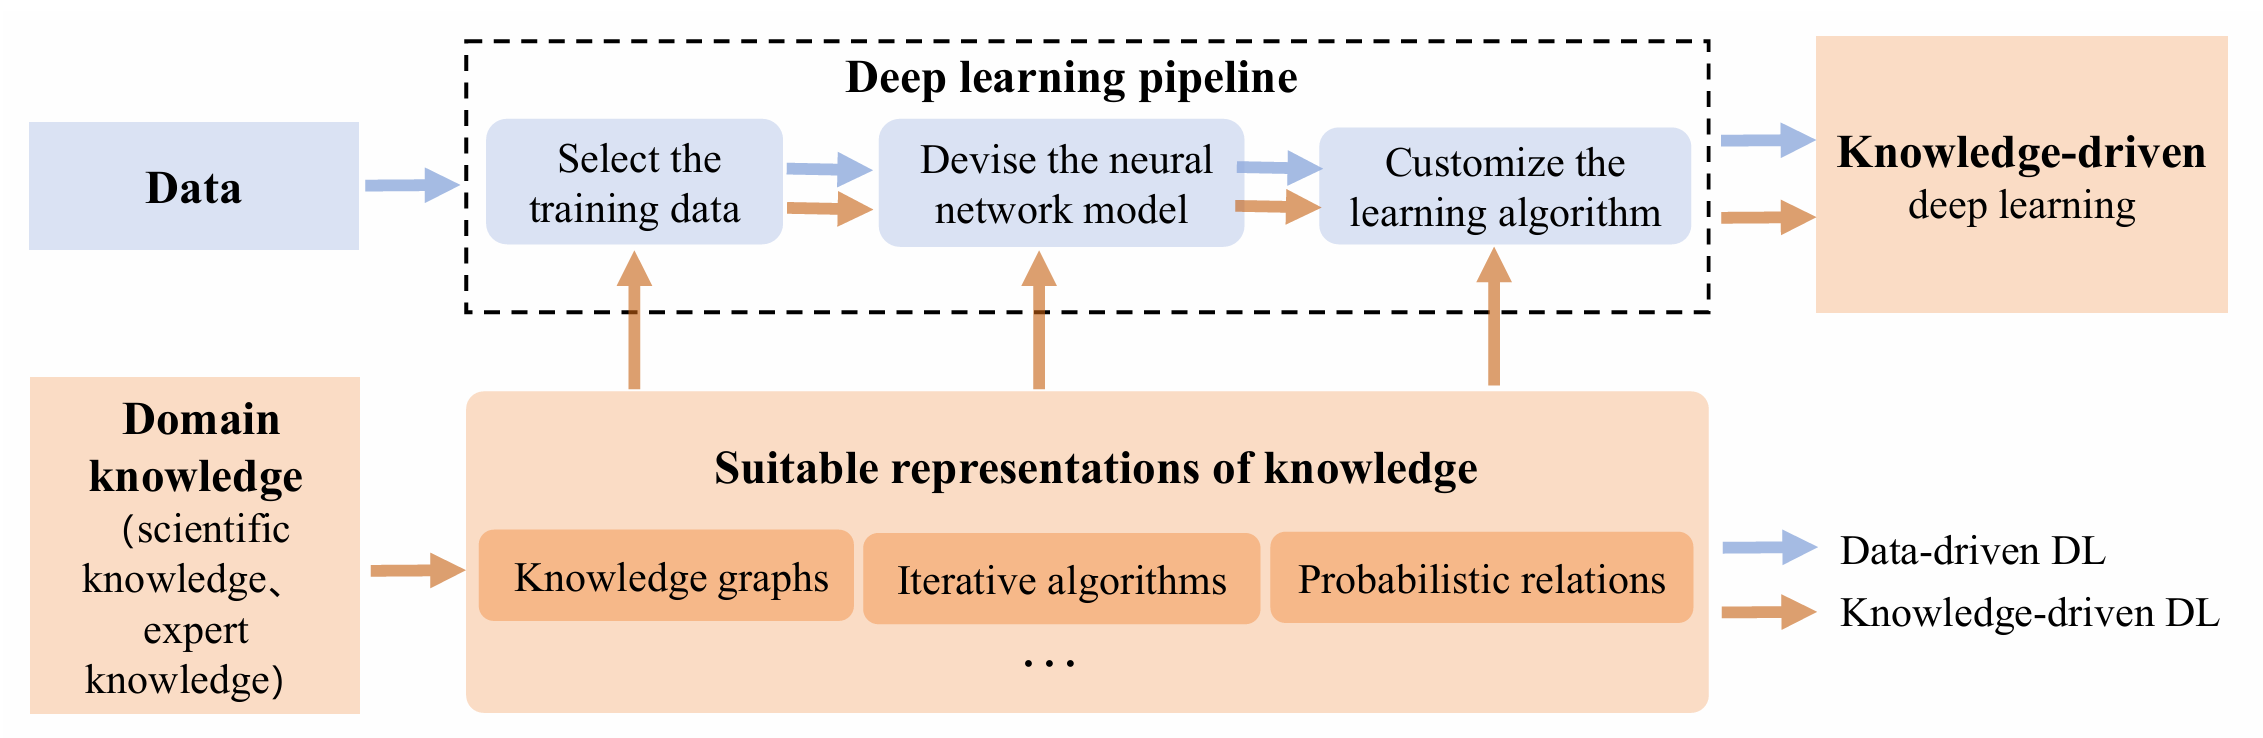
\includegraphics[width=0.9\linewidth]{./Pic/ComprehensiveSurvey_concepts_fig5}
   	\caption[\lofimage{./Pic/ComprehensiveSurvey_concepts_fig5} طبقه‌بندی دانش در شبکه‌های بی‌سیم شامل، دسته‌بندی دانش، نمایش‌دانش و مثال‌های رایج]{طبقه‌بندی دانش در شبکه‌های بی‌سیم شامل، دسته‌بندی دانش، نمایش‌دانش و مثال‌های رایج\cite{ComprehensiveSurvey}}
   	\label{concepts:fig5}
 \end{figure}
\gls{Knowledge-Driven Deep Learning}
 روشی است که در آن دانش دامنه خاص ارتباطات به صورت صریح ادغام می‌شود تا داده‌های آموزشی ناکافی را تقویت کرده و طراحی مدل شبکه عصبی و الگوریتم‌های یادگیری را هدایت کند
(\autoref{concepts:fig5}).
 این دانشِ یکپارچه‌شده، مستقل از داده‌های آموزشی اصلی برچسب‌گذاری شده است. 
\gls{Knowledge-Driven Deep Learning}
  به نظام‌فکری 
\gls{ante-hoc explainability}
   تعلق دارد، به این معنی که قابلیت تفسیر از همان ابتدای طراحی یا فرآیند یادگیری مدل تعبیه می‌شود. این ویژگی در شبکه‌های بی‌سیم با الزامات ایمنی-بحرانی، بسیار حیاتی است.‬
‫مسئله اساسی در 
\gls{Knowledge-Driven Deep Learning}
 چگونگی تعبیه مؤثر دانش در شبکه‌های عصبی است. یک طبقه‌بندی ساختاریافته از رویکردهای یکپارچه‌سازی دانش، بر اساس این که دانش به کدام یک از اجزای خط لوله 
\gls{Deep Learning}
  وارد می‌شود، ارائه شده است: این رویکردها شامل انتخاب مدل شبکه عصبی، سفارشی‌سازی مدل شبکه عصبی، ساختار تلفیق دانش و داده، طراحی 
\gls{Loss Function}،
   و پیکربندی 
\gls{Hyperparameter}   
    است.‬
    
‫بخش آخر، سفارشی‌سازی مدل و 
\gls{Deep Unfolding}
است.
‫سفارشی‌سازی مدل شبکه عصبی از 
\gls{Domain Knowledge}
 برای تنظیم مدل‌های 
\gls{Deep Neural Network}
 با هدف افزایش 
\gls{Interpretability}
  و انطباق‌پذیری استفاده می‌کند. این رویکرد به کاهش تعداد داده‌های آموزشی مورد نیاز و کاهش بار محاسباتی در آموزش آفلاین کمک می‌کند. این سفارشی‌سازی به سه دسته تقسیم می‌شود. طراحی زیرساختار، طراحی کل ساختار و شبکه‌های عصبی ترکیبی ساختار-محور.‬
‫در 
\gls{Substructure Design}،
 دانش در اجزای محلی شبکه مانند لایه خروجی یا تابع فعال‌سازی گنجانده می‌شود تا تضمین کند خروجی‌ها به محدودیت‌های عملیاتی خاص مسئله پایبند هستند. به‌عنوان مثال، در مسائ 
\gls{Beamforming}
  مقید 
\lr{MISO}،
 از یک 
\gls{Projection Function}
  خاص در لایه خروجی استفاده می‌شود تا مطمئن شویم خروجی در ناحیه امکان‌پذیر قرار می‌گیرد.‬
‫طراحی کل ساختار یا همان 
\gls{Algorithm Unfolding}،
 یک روش قدرتمند و مدل-محور است که دانش مربوط به الگوریتم‌های تکرارشونده اثبات شده را در کل ساختار شبکه عصبی تعبیه می‌کند. این روش، یک الگوریتم تکرارشونده مرسوم که از راه‌حل‌های نظری بهینه‌سازی شبکه مشتق شده است، را برای تعداد ثابتی از تکرارها باز می‌کند و هر تکرار را به عنوان یک لایه در 
\gls{Deep Neural Network}
  در نظر می‌گیرد.‬
\gls{Deep Unfolding}،
 ساختار و منطق الگوریتم اصلی بهینه‌سازی را حفظ می‌کند و در عین حال پارامترهای ثابت الگوریتم را به پارامترهای انعطاف‌پذیر و قابل یادگیری در شبکه عصبی تبدیل می‌نماید. این رویکرد ساختار لایه‌ای قابل تفسیری را فراهم می‌کند که در آن هر لایه تقریباً متناظر با یک مرحله از الگوریتم تکرارشونده مدل-محور است.‬
 
از آنجا که تعداد لایه‌ها یعنی تعداد تکرارها در مدل‌های 
\gls{Deep Unfolding}
 ثابت است، این مدل‌ها دارای پیچیدگی محاسباتی ثابت و از پیش تعریف‌شده‌ای هستند. این ویژگی به زمان 
\gls{Inference}
 سریع و قابل اعتماد به ویژه در کاربردهای 
\gls{Real-Time}
  می‌انجامد.‬ با ادغام صریح 
\gls{Domain Knowledge}
   در معماری،
\gls{Interpretability}   
    شبکه بهبود می‌یابد. همچنین، این روش‌ها 
\glspl{Trainable Parameter}
     کمتری نسبت به شبکه‌های جعبه سیاه عمومی دارند، که در نتیجه به مجموعه داده‌های آموزشی کمتری نیاز دارند.‬
\gls{Deep Unfolding}
به طور گسترده برای حل مسائل پردازش سیگنال مانند آشکارسازی سیگنال، تخمین کانال و طراحی 
\gls{Beamforming}
 و مدیریت منابع مانند تخصیص توان با استفاده از الگوریتم‌هایی نظیر 
\gls{WMMSE}
  یا 
\gls{PGD}/\gls{ADMM}
   به کار رفته است.‬ ساختار تلفیق دانش و داده و طراحی
\gls{Loss Function}
‫ساختار تلفیق دانش و داده یک نظام‌فکری ترکیبی است که در آن روش‌های نظری مدل-محور و شبکه‌های عصبی داده-محور به‌طور صریح و همکارانه برای حل مسائل بهینه‌سازی استفاده می‌شوند.

 این ساختارها عمدتاً دانش علمی یا راه‌حل‌های نظری را به‌عنوان منبع اصلی دانش خود به کار می‌گیرند. این تلفیق می‌تواند به صورت ترتیبی یا موازی انجام شود.‬
در حالت ترتیبی، بخش‌های دانش و داده به صورت متوالی عمل می‌کنند. این حالت خود به دو ساختار فرعی تقسیم می‌شود.‬‫ نخست 
\gls{Mixing Structure}
 بوده که در آن مسئله اصلی به چندین زیرمسئله مرتبط تقسیم می‌شود. بخش‌های دانش به زیرمسائلی که راه‌حل‌های تحلیلی بهینه یا الگوریتم‌های نظری با پیچیدگی پایین دارند، می‌پردازند و بخش‌های داده زیرمسائلی را که روابط نگاشتی با ابعاد بالا یا مدل‌سازی دشوار دارند، حل می‌کنند.‬
دوم 
\gls{Refinement Structure}
است که بخش دانش یک راه‌حل تقریبی اولیه بر اساس مدل‌های نظری تعمیم‌یافته ارائه می‌دهد و سپس بخش داده با استفاده از داده‌های دنیای واقعی، این راه‌حل اولیه را پالایش می‌کند. این استفاده از راه‌حل‌های اولیه به‌طور قابل توجهی نیاز به تعداد نمونه‌های داده آموزشی برای بخش‌های داده را کاهش می‌دهد. مثال‌های کاربردی آن شامل تخمین کانال که یک تخمین‌گر مرسوم 
\gls{LS}
 یک راه‌حل اولیه برای پالایش توسط یک 
\gls{Deep Neural Network}
  ارائه می‌دهد و آشکارسازی سیگنال است.‬
‫طراحی 
\gls{Loss Function}
 دانش‌محور روشی است که در آن 
\gls{Domain Knowledge}
  به صورت عبارت‌های اضافی فاقد برچسب در 
\gls{Loss Function}
   تعبیه می‌شود. این عبارات معمولاً از شناخت روش‌شناسی مدل‌سازی وظایف بی‌سیم و درک جامع از این وظایف نشأت می‌گیرند. هدف از این رویکرد، ترکیب یادگیری از داده‌های تجربی و دانش نظری برای بهبود قابلیت تعمیم و انطباق مدل است.‬
   
\gls{Constraint-Specific Loss Function}
نوعی از 
\gls{Loss Function}
است که دانش مربوط به محدودیت‌های ذاتی مسائل بهینه‌سازی را در 
\gls{Loss Function}
 گنجانده و با اعمال جریمه بر نقض محدودیت‌ها، فرآیند یادگیری را هدایت می‌کند. این رویکرد برای مدیریت مسائل با محدودیت‌های پیچیده از طریق شبکه‌های عصبی قدرتمند، روشی مؤثر است. یک مثال کلیدی، 
\gls{Primal-Dual Learning}
  است که با الهام از روش‌های 
\gls{Lagrange Duality}،
   محدودیت‌های پیچیده را به عنوان عبارت‌های جریمه خطی اضافی در 
\gls{Loss Function}
    گنجانده و بدین ترتیب یادگیری را هدایت می‌کند. همچنین، برای محدودیت‌های جمع خطی ساده، می‌توان محدودیت‌ها را با استفاده از توابع فعال‌سازی در 
\gls{Loss Function}
     تبدیل و اعمال کرد.‬
‫پیکربندی 
\glspl{Hyperparameter}
 دانش‌محور نیز از دانش قبلی برای تنظیم پارامترهای اولیه، ضریب‌های وزن‌دهی، و نرخ‌های یادگیری استفاده می‌کند. این کار به تسریع فرآیند آموزش و دستیابی به عملکرد قوی‌تر کمک می‌کند. به‌عنوان مثال، در الگوریتم‌هایی که از طریق 
\gls{Deep Unfolding}
  حل می‌شوند، پارامترهای اولیه شبکه‌های گسترش داده شده می‌توانند از راه‌حل‌های الگوریتم‌های تکرارشونده نظری که بخشی از 
\gls{Domain Knowledge}
  هستند به ارث برده شوند و این مقداردهی اولیه عملکرد مدل را به طور قابل توجهی بهبود می‌بخشد.‬

\begin{comment}
در سال‌های اخیر، رشد بی‌سابقه‌ی فناوری‌های هوش مصنوعی و یادگیری عمیق موجب تحولی بنیادین در حوزه‌ی ارتباطات بی‌سیم شده است. با ظهور نسل ششم شبکه‌های ارتباطی (6G)، نیاز به سیستم‌هایی که بتوانند تصمیم‌گیری‌های پیچیده و بلادرنگ انجام دهند بیش از هر زمان دیگری احساس می‌شود. در این مسیر، روش‌های یادگیری داده‌محور مانند \textit{Deep Learning} توانسته‌اند سهم بزرگی در ارتقای عملکرد لایه‌های مختلف شبکه ایفا کنند، اما همچنان با چالش‌هایی مانند نیاز به داده‌های فراوان، عدم تفسیرپذیری و ضعف در تعمیم به شرایط جدید مواجه‌اند. برای رفع این محدودیت‌ها، مفاهیم \textit{Model-Driven Learning} و به‌ویژه \textit{Deep Unfolding} مطرح شده‌اند که هدف آن‌ها ادغام دانش حوزه و الگوریتم‌های تحلیلی سنتی با قدرت یادگیری داده‌محور شبکه‌های عصبی است. این روش‌ها به‌طور ویژه در زمینه‌ی پردازش سیگنال، تخصیص منابع، برآورد کانال و بهینه‌سازی لایه‌ی فیزیکی شبکه‌های 6G نقش حیاتی دارند.

درک جایگاه \textit{Deep Unfolding} مستلزم شناخت تمایز میان سه پارادایم اصلی در یادگیری برای شبکه‌های بی‌سیم است: روش‌های مبتنی بر مدل (Model-Based)، روش‌های داده‌محور (Data-Driven) و روش‌های ترکیبی یا دانشی (Knowledge-Driven). در روش‌های مبتنی بر مدل، مسائل ارتباطی با استفاده از نظریه‌های ریاضی و قوانین فیزیکی مدل‌سازی می‌شوند. الگوریتم‌هایی مانند \textit{Water-Filling} یا \textit{WMMSE} نمونه‌هایی از این رویکرد هستند که پاسخ‌های بهینه یا نزدیک به بهینه ارائه می‌دهند، اما در مقابل پیچیدگی محاسباتی بالایی دارند و در شرایط متغیر واقعی به‌سختی قابل پیاده‌سازی‌اند. در طرف مقابل، روش‌های داده‌محور با تکیه بر شبکه‌های عصبی و داده‌های آموزشی گسترده تلاش می‌کنند رابطه‌ی مستقیم بین ورودی‌ها و خروجی‌های بهینه را یاد بگیرند. این رویکرد، اگرچه در بسیاری از کاربردها مانند تشخیص سیگنال، تخصیص توان یا پیش‌بینی کیفیت کانال موفق بوده، اما به‌دلیل ماهیت «جعبه‌سیاه» خود فاقد تفسیرپذیری و تضمین نظری عملکرد است. اینجاست که مفهوم یادگیری دانشی و به‌ویژه \textit{Deep Unfolding} به‌عنوان پلی میان دو جهان مدل‌محور و داده‌محور ظهور می‌کند.

روش \textit{Deep Unfolding} اساساً بر ایده‌ی بازنویسی الگوریتم‌های تکراری مرسوم در قالب شبکه‌های عصبی عمیق استوار است. در بسیاری از الگوریتم‌های بهینه‌سازی، مسئله به‌صورت تکراری و گام‌به‌گام حل می‌شود تا به جواب نهایی همگرا گردد. ایده‌ی اصلی در \textit{Deep Unfolding} این است که هر تکرار از الگوریتم سنتی را می‌توان به‌صورت یک لایه در شبکه‌ی عصبی مدل کرد و پارامترهای کلیدی مانند گام یادگیری، ضرایب وزن، یا پارامترهای تنظیمی را به‌صورت داده‌محور آموزش داد. در نتیجه، شبکه‌ی نهایی ترکیبی از منطق صریح الگوریتمی و قدرت تطبیقی یادگیری است. چنین مدلی ضمن حفظ تفسیرپذیری ذاتی الگوریتم اولیه، از انعطاف‌پذیری داده‌محور در شرایط واقعی نیز بهره‌مند می‌شود.

برای مثال، در مسئله‌ی برآورد کانال در سیستم‌های \textit{MIMO}، الگوریتم‌های سنتی مانند \textit{Iterative Shrinkage Thresholding Algorithm (ISTA)} با تکرارهای متوالی ضرایب کانال را به‌دست می‌آورند. با بازگشایی این الگوریتم در قالب \textit{Deep Unfolding}، هر تکرار ISTA به‌عنوان یک لایه در شبکه‌ی عصبی در نظر گرفته می‌شود و پارامترهای تنظیمی در طول آموزش به‌صورت خودکار بهینه می‌شوند. این کار منجر به همگرایی سریع‌تر، دقت بالاتر و کاهش نیاز به تنظیمات دستی می‌گردد. نمونه‌ی معروف این ساختار \textit{LISTA} است که از بازگشایی ISTA مشتق شده و در بسیاری از کاربردهای مخابراتی و پردازش سیگنال استفاده می‌شود.

یکی از مزیت‌های بنیادی \textit{Deep Unfolding} نسبت به روش‌های صرفاً داده‌محور، قابلیت تفسیرپذیری ذاتی آن است. در حالی که شبکه‌های عصبی عمیق معمولی مانند \textit{CNN} یا \textit{RNN} تنها از داده یاد می‌گیرند و روابط داخلی آن‌ها غالباً غیرقابل تحلیل است، مدل‌های بازگشایی‌شده بر مبنای ساختار الگوریتمی بنا شده‌اند و هر لایه معادل یک گام محاسباتی مشخص در فرایند بهینه‌سازی است. از این رو، تغییرات در پارامترها یا عملکرد هر بخش از شبکه می‌تواند به‌طور مستقیم به تئوری و منطق اصلی الگوریتم مرتبط شود. این ویژگی برای شبکه‌های بی‌سیم نسل ششم که نیازمند اعتماد، قابلیت توضیح و پایداری در محیط‌های بحرانی‌اند اهمیت حیاتی دارد.

در بستر شبکه‌های 6G، پیچیدگی ارتباطات و تنوع سناریوها به‌گونه‌ای است که روش‌های مرسوم بهینه‌سازی دیگر پاسخ‌گو نیستند. شبکه‌های 6G نه‌تنها باید ارتباطات داده را مدیریت کنند، بلکه باید حس‌گری، مکان‌یابی، تصمیم‌گیری و حتی استنتاج معنایی را نیز یکپارچه سازند. در چنین محیطی، \textit{Deep Unfolding} می‌تواند با ترکیب دانش فیزیکی شبکه (مانند مدل کانال یا محدودیت توان) و قدرت یادگیری عمیق، راه‌حلی کارآمد و تفسیرپذیر برای بهینه‌سازی ارائه دهد. برای نمونه، در مسئله‌ی تخصیص توان در ارتباطات \textit{Non-Orthogonal Multiple Access (NOMA)}، استفاده از \textit{Deep Unfolding} باعث می‌شود ساختار بازگشتی الگوریتم‌های \textit{WMMSE} درون شبکه‌ی عصبی تعبیه شود. در این حالت، شبکه نه‌تنها از داده‌ها الگو می‌گیرد بلکه اصول فیزیکی و ریاضی مسئله را نیز رعایت می‌کند، که نتیجه‌ی آن کارایی بالاتر و نیاز کمتر به داده‌های آموزشی است.

از منظر ریاضی، فرایند \textit{Deep Unfolding} را می‌توان به‌صورت بازنمایی نگاشت تابعی الگوریتم تکراری در قالب شبکه‌ای با لایه‌های قابل یادگیری تعبیر کرد. در هر لایه، ورودی‌ها بر اساس روابط مشتق‌شده از الگوریتم اصلی به‌روزرسانی می‌شوند و برخی پارامترها مانند ضرایب وزنی یا فاکتورهای منظم‌سازی به‌صورت داده‌محور تنظیم می‌گردند. خروجی نهایی شبکه معمولاً برآوردی از متغیر بهینه یا تصمیم مطلوب در مسئله‌ی مخابراتی است. برای جلوگیری از بیش‌برازش و تضمین پایداری، در بسیاری از کارها از قیود فیزیکی شبکه مانند محدودیت توان، نرخ داده، یا خطای برآورد در تابع زیان شبکه استفاده می‌شود. این امر موجب می‌شود که مدل علاوه‌بر دقت بالا، از لحاظ عملکرد عملی نیز منطبق با واقعیت‌های فیزیکی سیستم باقی بماند.

یکی از ویژگی‌های مهم \textit{Deep Unfolding} آن است که معمولاً به داده‌های آموزشی کمتری نسبت به مدل‌های کاملاً داده‌محور نیاز دارد. دلیل این امر آن است که بخش قابل‌توجهی از ساختار و دانش مسئله از قبل در شبکه رمزگذاری شده است. این مسئله به‌ویژه در شبکه‌های بی‌سیم که گردآوری داده‌های واقعی هزینه‌بر و زمان‌بر است، اهمیت ویژه‌ای دارد. از سوی دیگر، استفاده از ساختار الگوریتمی باعث می‌شود فرآیند آموزش سریع‌تر همگرا شود و مدل نهایی پایداری بیشتری نسبت به تغییرات شرایط محیطی داشته باشد.

در کاربردهای لایه‌ی فیزیکی شبکه‌های 6G، \textit{Deep Unfolding} در حوزه‌های متعددی به‌کار رفته است: از تشخیص سیگنال و برآورد کانال گرفته تا طراحی پرکدرها (precoders)، تخصیص توان، رمزگشایی کدهای تصحیح خطا و ادغام حس‌گر و ارتباط (ISAC). در مسئله‌ی تشخیص سیگنال، شبکه‌های بازگشایی‌شده توانسته‌اند با ترکیب الگوریتم‌های تکراری مانند \textit{Approximate Message Passing (AMP)} با لایه‌های یادگیری، عملکردی نزدیک به بهینه با پیچیدگی بسیار کمتر ارائه دهند. در برآورد کانال نیز شبکه‌های مبتنی بر \textit{Deep Unfolding} توانسته‌اند دقت برآورد را با استفاده از اطلاعات ساختاری کانال افزایش دهند. در طراحی پرکدرها و تخصیص منابع، از بازگشایی الگوریتم‌های \textit{WMMSE}، \textit{Projected Gradient Descent (PGD)} و \textit{ADMM} برای ساخت شبکه‌های تفسیرپذیر و کارآمد استفاده شده است.

یکی دیگر از زمینه‌های نوظهور، کاربرد \textit{Deep Unfolding} در ادغام حس‌گری و ارتباط (\textit{Integrated Sensing and Communication}) است. در این سناریو، سیستم باید هم‌زمان وظایف ارسال داده و دریافت اطلاعات محیطی را انجام دهد. این امر مستلزم طراحی سیگنال‌هایی با قابلیت تفکیک بالا و تداخل کم است. استفاده از \textit{Deep Unfolding} در این حوزه باعث می‌شود ساختار بهینه‌سازی سیگنال و تخمین پارامترها به‌صورت لایه‌به‌لایه درون شبکه پیاده شود، به‌گونه‌ای که مدل بتواند میان کارایی ارتباطی و دقت حس‌گری تعادل برقرار کند.

در مقایسه با سایر رویکردهای ترکیبی مانند \textit{Physics-Informed Neural Networks (PINNs)} یا \textit{Knowledge-Driven DL}، روش \textit{Deep Unfolding} مزیت ساختاری دارد زیرا فرآیند یادگیری آن از الگوریتم‌های موجود استخراج می‌شود و در نتیجه، مسیر بهینه‌سازی آن از لحاظ ریاضی قابل تحلیل است. به‌عبارت دیگر، \textit{Deep Unfolding} نه‌تنها از دانش دامنه استفاده می‌کند، بلکه آن را به‌صورت صریح در معماری شبکه پیاده‌سازی می‌نماید. این ویژگی، آن را برای سیستم‌های بحرانی مانند شبکه‌های خودران، مخابرات صنعتی، یا ارتباطات هواپایه ایده‌آل می‌سازد که در آن‌ها نیاز به اطمینان و تفسیرپذیری بالا وجود دارد.

افزون بر این، توسعه‌ی \textit{Deep Unfolding} در تعامل با فناوری‌هایی نظیر \textit{Graph Neural Networks (GNNs)} زمینه‌ی نوینی را در مدل‌سازی شبکه‌های بی‌سیم باز کرده است. از آنجا که توپولوژی ارتباطات اغلب به‌صورت گرافی نمایش داده می‌شود، ادغام ساختار گراف با بازگشایی الگوریتمی موجب بهبود یادگیری روابط مکانی میان گره‌ها و تقویت عملکرد در تخصیص منابع توزیع‌شده می‌شود. ترکیب \textit{Deep Unfolding} با GNN، که در برخی منابع با عنوان \textit{WUGNN} معرفی شده، نشان داده است که می‌توان الگوریتم‌های سنتی مانند \textit{WMMSE} را در قالب گرافی تفسیرپذیر با قابلیت یادگیری بازنمایی کرد.

در نهایت، می‌توان گفت \textit{Deep Unfolding} یکی از مسیرهای کلیدی در تحول شبکه‌های هوشمند آینده است، زیرا پلی میان نظریه و داده برقرار می‌کند. در حالی که روش‌های سنتی همچنان از نظر بنیان‌های ریاضی دقیق و قابل تحلیل‌اند و شبکه‌های یادگیری عمیق از نظر قدرت مدل‌سازی داده‌ها برتری دارند، \textit{Deep Unfolding} تلاش می‌کند بهترین ویژگی‌های هر دو را در قالبی واحد گردآورد. با پیشرفت 6G و حرکت به سوی سیستم‌های خودآموز و خودسازمان‌ده، این رویکرد می‌تواند چارچوبی فراهم آورد که در آن مدل‌های یادگیری نه‌تنها از داده بیاموزند بلکه دانش فیزیکی و الگوریتمی سیستم را نیز در خود جای دهند. چنین هم‌افزایی، مسیر دستیابی به شبکه‌های واقعاً هوشمند، تفسیرپذیر و کارآمد را هموار خواهد کرد.
\end{comment}

\begin{comment}
\label{chap:concepts}
در ابتدای هر فصل از پایان‌نامه، سعی کنید نخست بدون شروع هرگونه 
\lr{Section}، 
به طور خلاصه بگویید که قرار است در این فصل در مورد چه چیزی صحبت کنید. به عنوان مثال در این فصل، نخست در 
\autoref{sec:boostanenv}،
در مورد محیط‌های مختلفی که می‌توانید در استایل بوستان از آن استفاده کنید، صحبت خواهیم کرد. سپس در 
\autoref{sec:codeintext}،
در مورد نحوه وارد کردن یک کد در متن سخن به میان خواهد آمد. 

\section{محیط‌های مختلف در استایل بوستان}\index{محیط}
\label{sec:boostanenv}
‎\ptext[1]
\subsection{محیط نکات}
\begin{note}
شهر مردگان، شهر انسان های «بی دفاع» است. این تعبیر اقتباس از قرآن کریم است که «غیبت» را خوردن گوشت «مرده» خوانده است. 
\begin{equation}
A = B + \sin (x)
\end{equation}
در تفاسیر آمده است که خداوند «انسان بی دفاع» را که به دلیل عدم حضور در مجلس بدگویی نمی تواند از خود دفاع کند، «مرده» دانسته است. پس آنجا که نسبت های ناروا دادن مباح، و دفاع کردن ممنوع است، در حقیقت «شهر مردگان» است.
\end{note}
‎\ptext[2]
\begin{problem}
شهر مردگان، شهر انسان های «بی دفاع» است. این تعبیر اقتباس از قرآن کریم است که «غیبت» را خوردن گوشت «مرده» خوانده است . در تفاسیر آمده است که خداوند «انسان بی دفاع» را که به دلیل عدم حضور در مجلس بدگویی نمی تواند از خود دفاع کند، «مرده» دانسته است. پس آنجا که نسبت های ناروا دادن مباح، و دفاع کردن ممنوع است، در حقیقت «شهر مردگان» است.


\end{problem}
‎\ptext[3]
\begin{refer}
شهر مردگان، شهر انسان های «بی دفاع» است. این تعبیر اقتباس از قرآن کریم است که «غیبت» را خوردن گوشت «مرده» خوانده است.
\begin{latin}
\lstset{numbers=none,frame=none}
\begin{lstlisting}
for i:=maxint to 0 do
begin
{ do nothing }
end;
\end{lstlisting}
\end{latin}
  در تفاسیر آمده است که خداوند «انسان بی دفاع» را که به دلیل عدم حضور در مجلس بدگویی نمی تواند از خود دفاع کند، «مرده» دانسته است. پس آنجا که نسبت های ناروا دادن مباح، و دفاع کردن ممنوع است، در حقیقت «شهر مردگان» است.
\end{refer}

\begin{info}
شهر مردگان، شهر انسان های «بی دفاع» است. این تعبیر اقتباس از قرآن کریم است که «غیبت» را خوردن گوشت «مرده» خوانده است . 
در تفاسیر آمده است که خداوند «انسان بی دفاع» را که به دلیل عدم حضور در مجلس بدگویی نمی تواند از خود دفاع کند، «مرده» دانسته است. پس آنجا که نسبت های ناروا دادن مباح، و دفاع کردن ممنوع است، در حقیقت «شهر مردگان» است.
\begin{equation}
A = B + \sin (x)
\end{equation}
\end{info}

\index{نکته}
\begin{warning}{نکات مهم}
شهر مردگان، شهر انسان های «بی دفاع» است. این تعبیر اقتباس از قرآن کریم است که «غیبت» را خوردن گوشت «مرده» خوانده است . در تفاسیر آمده است که خداوند «انسان بی دفاع» را که به دلیل عدم حضور در مجلس بدگویی نمی تواند از خود دفاع کند، «مرده» دانسته است. پس آنجا که نسبت های ناروا دادن مباح، و دفاع کردن ممنوع است، در حقیقت «شهر مردگان» است.
\end{warning}


\begin{goal}{نکات مهم}
شهر مردگان، شهر انسان های «بی دفاع» است. این تعبیر اقتباس از قرآن کریم است که «غیبت» را خوردن گوشت «مرده» خوانده است . 

در تفاسیر آمده است که خداوند «انسان بی دفاع» را که به دلیل عدم حضور در مجلس بدگویی نمی تواند از خود دفاع کند، «مرده» دانسته است.

  پس آنجا که نسبت های ناروا دادن مباح، و دفاع کردن ممنوع است، در حقیقت «شهر مردگان» است.
\end{goal}

\subsection{محیط‌های ریاضی}
کارکرد لاتک مبتنی بر این اندیشه است که نویسندگان باید قادر باشند بر نوشتن در درون ساختار منطقی متن‌شان تمرکز کنند، نه اینکه وقت خود را برای کار کردن بر روی جزئیات شکل‌دهی صرف کنند. 
\begin{ntdefinition}
شهر مردگان، شهر انسان های «بی دفاع» است. 
\end{ntdefinition}
کارکرد لاتک مبتنی بر این اندیشه است که نویسندگان باید قادر باشند بر نوشتن در درون ساختار منطقی متن‌شان تمرکز کنند، نه اینکه وقت خود را برای کار کردن بر روی جزئیات شکل‌دهی صرف کنند. 
\begin{ntdefinition}
شهر مردگان، شهر انسان های «بی دفاع» است. 
\end{ntdefinition}
کارکرد لاتک مبتنی بر این اندیشه است که نویسندگان باید قادر باشند بر نوشتن در درون ساختار منطقی متن‌شان تمرکز کنند، نه اینکه وقت خود را برای کار کردن بر روی جزئیات شکل‌دهی صرف کنند. 
\begin{ntexample}
شهر مردگان، شهر انسان های «بی دفاع» است. 
\end{ntexample}
کارکرد لاتک مبتنی بر این اندیشه است که نویسندگان باید قادر باشند بر نوشتن در درون ساختار منطقی متن‌شان تمرکز کنند، نه اینکه وقت خود را برای کار کردن بر روی جزئیات شکل‌دهی صرف کنند. 
\begin{ntexample}
شهر مردگان، شهر انسان های «بی دفاع» است. 
\end{ntexample}
\begin{ntsolution}
شهر مردگان، شهر انسان های «بی دفاع» است. این تعبیر اقتباس از قرآن کریم است که «غیبت» را خوردن گوشت «مرده» خوانده است . در تفاسیر آمده است که خداوند «انسان بی دفاع» را که به دلیل عدم حضور در مجلس بدگویی نمی تواند از خود دفاع کند، «مرده» دانسته است. پس آنجا که نسبت های ناروا دادن مباح، و دفاع کردن ممنوع است، در حقیقت «شهر مردگان» است.
\end{ntsolution}
کارکرد لاتک مبتنی بر این اندیشه است که نویسندگان باید قادر باشند بر نوشتن در درون ساختار منطقی متن‌شان تمرکز کنند، نه اینکه وقت خود را برای کار کردن بر روی جزئیات شکل‌دهی صرف کنند. 

\begin{ntpoint}

شهر مردگان، شهر انسان های «بی دفاع» است. شهر مردگان، شهر انسان های «بی دفاع» است. شهر مردگان، شهر انسان های «بی دفاع» است. شهر مردگان، شهر انسان های «بی دفاع» است. 
\end{ntpoint}
کارکرد لاتک مبتنی بر این اندیشه است که نویسندگان باید قادر باشند بر نوشتن در درون ساختار منطقی متن‌شان تمرکز کنند، نه اینکه وقت خود را برای کار کردن بر روی جزئیات شکل‌دهی صرف کنند. 

کارکرد لاتک مبتنی بر این اندیشه است که نویسندگان باید قادر باشند بر نوشتن در درون ساختار منطقی متن‌شان تمرکز کنند، نه اینکه وقت خود را برای کار کردن بر روی جزئیات شکل‌دهی صرف کنند. 

\begin{nttheorem}
شهر مردگان، شهر انسان های «بی دفاع» است. این تعبیر اقتباس از قرآن کریم است که «غیبت» را خوردن گوشت «مرده» خوانده است . در تفاسیر آمده است که خداوند «انسان بی دفاع» را که به دلیل عدم حضور در مجلس بدگویی نمی تواند از خود دفاع کند، «مرده» دانسته است. پس آنجا که نسبت های ناروا دادن مباح، و دفاع کردن ممنوع است، در حقیقت «شهر مردگان» است.
\end{nttheorem}
\begin{nttheorem}
شهر مردگان، شهر انسان های «بی دفاع» است. این تعبیر اقتباس از قرآن کریم است که «غیبت» را خوردن گوشت «مرده» خوانده است . در تفاسیر آمده است که خداوند «انسان بی دفاع» را که به دلیل عدم حضور در مجلس بدگویی نمی تواند از خود دفاع کند، «مرده» دانسته است. پس آنجا که نسبت های ناروا دادن مباح، و دفاع کردن ممنوع است، در حقیقت «شهر مردگان» است.
\end{nttheorem}
\begin{proof}
شهر مردگان، شهر انسان های «بی دفاع» است. این تعبیر اقتباس از قرآن کریم است که «غیبت» را خوردن گوشت «مرده» خوانده است . در تفاسیر آمده است که خداوند «انسان بی دفاع» را که به دلیل عدم حضور در مجلس بدگویی نمی تواند از خود دفاع کند، «مرده» دانسته است. پس آنجا که نسبت های ناروا دادن مباح، و دفاع کردن ممنوع است، در حقیقت «شهر مردگان» است.
\end{proof}

\begin{lemma}
شهر مردگان، شهر انسان های «بی دفاع» است. این تعبیر اقتباس از قرآن کریم است که «غیبت» را خوردن گوشت «مرده» خوانده است . در تفاسیر آمده است که خداوند «انسان بی دفاع» را که به دلیل عدم حضور در مجلس بدگویی نمی تواند از خود دفاع کند، «مرده» دانسته است. پس آنجا که نسبت های ناروا دادن مباح، و دفاع کردن ممنوع است، در حقیقت «شهر مردگان» است.
\end{lemma}
\begin{lemmaproof}
شهر مردگان، شهر انسان های «بی دفاع» است. این تعبیر اقتباس از قرآن کریم است که «غیبت» را خوردن گوشت «مرده» خوانده است . در تفاسیر آمده است که خداوند «انسان بی دفاع» را که به دلیل عدم حضور در مجلس بدگویی نمی تواند از خود دفاع کند، «مرده» دانسته است. پس آنجا که نسبت های ناروا دادن مباح، و دفاع کردن ممنوع است، در حقیقت «شهر مردگان» است.
\end{lemmaproof}
\begin{ntremember}
شهر مردگان، شهر انسان های «بی دفاع» است. این تعبیر اقتباس از قرآن کریم است که «غیبت» را خوردن گوشت «مرده» خوانده است . در تفاسیر آمده است که خداوند «انسان بی دفاع» را که به دلیل عدم حضور در مجلس بدگویی نمی تواند از خود دفاع کند، «مرده» دانسته است. پس آنجا که نسبت های ناروا دادن مباح، و دفاع کردن ممنوع است، در حقیقت «شهر مردگان» است.
\end{ntremember}
\begin{ntproblems}
شهر مردگان، شهر انسان های «بی دفاع» است. این تعبیر اقتباس از قرآن کریم است که «غیبت» را خوردن گوشت «مرده» خوانده است . در تفاسیر آمده است که خداوند «انسان بی دفاع» را که به دلیل عدم حضور در مجلس بدگویی نمی تواند از خود دفاع کند، «مرده» دانسته است. پس آنجا که نسبت های ناروا دادن مباح، و دفاع کردن ممنوع است، در حقیقت «شهر مردگان» است.
\end{ntproblems}

\section{وارد کردن کد در متن}
\label{sec:codeintext}
مثالی از نوشتن کد مطلب درون یک نوشتار:

\begin{latin}
\lstinputlisting[language=Matlab]{Code/code3.m}
\end{latin}

در این مثال یک کد \lr{MATLAB} دیگر وارد می کنیم، با این تفاوت که می خواهیم یکسری از کلمات کلیدی را مشخص کنیم که لاتک آن ها را با رنگی به خصوصی نشان دهد. 
\begin{latin}
\lstset{emph={binornd},emphstyle=\color{Magenta}}
\lstinputlisting[language=Matlab, morekeywords={ksdensity}]{Code/prog3.m}
\end{latin}

مثالی دیگر از نوشتن کد مطلب در یک نوشتار. فقط در این حالت می خواهیم برخی از تنظیمات پیش فرض را که قبل از شروع نوشتار تعیین کرده ایم، تغییر دهیم. 
\begin{latin}
\lstinputlisting[numbers=right,language=Matlab, framexleftmargin=5mm, frame=shadowbox,rulesepcolor=\color{Yellow}]{Code/code4.m}
\end{latin}

در ضمن شما می توانید حتی در خود همین نوشتار اصلی خود کد مورد نظرتان را بنویسید. 
\begin{latin}
\begin{lstlisting}[mathescape=true]
// calculate  $a_{ij}$
$a_{ij} = a_{jj}/a_{ij} + \alpha$;
\end{lstlisting}
\end{latin}
\end{comment}